\documentclass[plain]{sigplanconf}
\usepackage{balance} % For balanced columns on the last page
\usepackage{amsmath}
\usepackage[T1]{fontenc}
\usepackage{lmodern}
\usepackage{graphicx}
\usepackage{amssymb}
\usepackage{tikz}
\usepackage{array}
\usepackage{longtable}
\usepackage{listings}
\usepackage{xcolor}
\usepackage[toc,page]{appendix}
\usepackage[
bookmarksopen,
bookmarksdepth=2,
breaklinks=true
]{hyperref}
\usepackage{natbib}
\setcitestyle{square,sort,comma,numbers}
\makeatletter
\def\BState{\State\hskip-\ALG@thistlm}
\makeatother

\makeatletter
\def\@copyrightspace{\relax}
\makeatother
%New colors defined below
\definecolor{eclipseStrings}{RGB}{42,0.0,255}
\definecolor{eclipseKeywords}{RGB}{127,0,85}
\colorlet{numb}{magenta!60!black}
\lstdefinelanguage{json}{
    basicstyle=\normalfont\ttfamily,
    commentstyle=\color{eclipseStrings}, % style of comment
    stringstyle=\color{eclipseKeywords}, % style of strings
    numbers=left,
    numberstyle=\scriptsize,
    stepnumber=1,
    numbersep=8pt,
    showstringspaces=false,
    breaklines=true,
    frame=lines,
    backgroundcolor=\color{gray}, %only if you like
    string=[s]{"}{"},
    comment=[l]{:\ "},
    morecomment=[l]{:"},
    literate=
    *{0}{{{\color{numb}0}}}{1}
    {1}{{{\color{numb}1}}}{1}
    {2}{{{\color{numb}2}}}{1}
    {3}{{{\color{numb}3}}}{1}
    {4}{{{\color{numb}4}}}{1}
    {5}{{{\color{numb}5}}}{1}
    {6}{{{\color{numb}6}}}{1}
    {7}{{{\color{numb}7}}}{1}
    {8}{{{\color{numb}8}}}{1}
    {9}{{{\color{numb}9}}}{1}
}
\begin{document}
\begin{figure}
		\centering
		
\includegraphics{sections/pictures-diagrams/PaperCoverSheet.pdf}
	\end{figure}
	\title{Simulating Africa's Internet Topology }
	%%\subtitle{Philosophy Invades Software Engineering}
	\authorinfo{Willie Macharia}
	{Department of Computer Science\linebreak University of Cape Town\linebreak South Africa}
	{September 2020}
	\maketitle
	\begin{abstract}
	Internet traffic originating from Africa and destined to Africa has been characterised with high latency. This has been due to the circuitous paths the intra-continent traffic follows. Many internet researchers have recommended that to solve this challenge, various African ISPs need to peer at local African IXPs. However, the question that arises from this recommendation is what is the best way the African ISPs can peer at local African IXPS and offer the best internet performance. The solution to this question is to first map the existing African internet topology and then perform topology simulation to evaluate performance of various routing and peering scenarios. 

    This paper presents the development and assessment of a web internet topology simulator. The developed simulator allows internet researchers to evaluate internet performance based on the peering scenario and given network conditions. Most of the existing simulators do not run on the web and depend on synthetic generated topology but the simulator discussed in this paper runs on the web and uses topology generated from real internet measurements. 


	\end{abstract}
	\begin{CCSXML}
		<ccs2012>
		<concept>
		 <concept_id>10003033.10003106.10003114</concept_id>
       <concept_desc>Networks~Overlay and other logical network structures</concept_desc>
       <concept_significance>500</concept_significance>
		</concept>
		</ccs2012>
	\end{CCSXML}
	\ccsdesc[500]{Networks~Overlay and other logical network structures}
	
	
	\keywords
	ISP Peering, IXP, Network Measurements,
	Internet Topology
	\section{Introduction}\label{sec:introduction}
Internet topology can be defined as the structure in which various internet components such as ISPs, routers, switches and end systems are connected to each other\cite{encyclopedia1}. In the last decade, internet connectivity has increased as many devices have been connected to the internet which in turn has led to rapid change of the internet topology. Oftenly, internet topology is a map where the nodes represent the various internet components and the links represent the interconnections between those components. To facilitate the topology mapping, topology discovery techniques are used to collect internet measurements from different internet measuring platforms\cite{Donnet2007}. These topology techniques are divided into two: passive techniques and active techniques.

Passive techniques use the BGP routing table to infer topology data that is used to map internet topology on AS-level and router level. Active techniques involve sending internet traffic to selected network destinations with an aim to collect topological data. The responses received from the destinations are then sampled and analysed to determine the routing path and the Round Trip Time(RTT) of the traffic\cite{Donnet2007}. 

Internet Exchange Points(IXPs) can be described as locations where ISPs and CDNs(Content Delivery Networks) meet and exchange internet traffic\cite{effectsofIXPS}. IXPs are important as they facilitate peering amongst ISPs\cite{effectsofIXPS}. Peering is a business relationship between ISPs where the ISPs agree to exchange internet traffic from each other. Peering reduces end to end traffic’s latency and improves the internet’s quality of service. 

According to AFRINIC\cite{Africanp74:online}, the African Regional Internet Registry, Africa had 46 IXPs spread across 34 countries by August 2020. Most of these IXPs remain underutilised as according to PeeringDB\cite{PeeringD7:online}, more than 60\% of these IXPs have less than 10 ISPs peering per IXP.  Most African ISPs have been found to peer at IXPs outside the continent. This has in turn affected the intra-continental traffic negatively as it experiences high end to end latency since the traffic is forced to be routed outside the continent so as to get to its destination \cite{africanet1}. According to Chavula \textit{et al} \cite{Africa2}, internet performance in Africa can be improved if peering of African ISPs is increased at African IXPs. To determine how best this peering can be done, various peering and routing  scenarios need to be simulated and tested using network simulators. 

\subsection{Project Objectives}
The objective of this project was to develop and create an online internet topology simulation platform that would evaluate how various ISPs could peer at Africa IXPs and how the internet performance affected would be affected. 

This paper describes the agile process of designing and creating the simulator and how the simulator was used to simulate the internet topology under various routing and peering conditions. The results from various scenarios are also described and discussed in the rest of the paper.  

	
\section{BACKGROUND}
 To simulate the mesh network of the internet, various network simulation techniques are used. These simulation techniques differs from each other depending on the nature of the simulator, the conditions under which the simulator runs on and also the type of initial topology that is used during simulation. Depending on the nature of the simulator, network simulation techniques can be described to be running on a web-based simulator or on a non-web simulator. Web based simulators are easier to use compared to non-web simulators as they don't require prior installation. Network simulation may use a synthetic network topology or non-synthetic topology. Synthetic topologies are generated from modelling the network from mathematical algorithms but non-synthetic topologies are generated from real measurements taken from the network. Due to the ever-changing nature of internet, it is not effective to use synthetic topologies to simulate the internet. It is important to run Internet measurements and use the data collected to generate the initial topology. Simulation results obtained from simulating non-synthetic topologies are more reliable compared to r5results obtained from simulating synthetic topologies.  
 
 Simulation of internet graphs involves adjusting the number of nodes or adjusting the number of edges \cite{Internetgraph} present on the graph. The adjustment can be done by removing or adding either nodes or the edges on the graph. The aim of such simulation is to test how the internet performance can be affected when different network conditions are introduced to internet topology. When a network condition is introduced, the topology is said to be under a certain scenario. To simulate the topology, the mapped topology is subjected to the condition which in turn changes the routing of the mapped nodes. Internet traffic is then sent from source to a selected destination and the link delay between the source and destination is measured and recorded. Internet topology mapped at AS-level may be simulated under the following conditions: adding an IXP node, adding links between nodes, removing links between nodes and removing nodes.  

\textbf{Adding an IXP node followed by adding links between nodes and the introduced IXP node:} This condition tests what could happen if an IXP is introduced at a certain location and some ISPs decide to connect through it.  During simulation, when an IXP node is added to the internet topology, selected nodes are then connected to the IXP. The node degree of the connected nodes increases and if some nodes are near the IXP, the link delay of traffic between these nodes is expected to decrease. The results obtained from this scenario are used to show what could be the effect of introducing an IXP node at a certain location. 

\textbf{Removing a link between two nodes:} This condition tests what could happen to the internet traffic flow if a link between two ISPs  is removed or goes down. During simulation, when a link between two nodes is removed, traffic flowing between the two nodes is expected to look for an alternative route. The link delay of the alternative route is then measured to indicate how the internet performance was affected by the link removal. 

\textbf{Removing node:} This condition tests what happens if one of the ISPs closes or ceases operations. During simulation, if a node is removed, its associated links are also removed. If any other nodes were connecting through the removed node, the internet traffic flow is expected to change as routing has been affected.  


\section{Related Work}\label{sec:Related Work}
%Are there any theories, concepts, terms, and ideas that may be unfamiliar to the target audience and will require you to provide any additional explanation?
%Any historical data that need to be shared in order to provide context on why the current issue emerged?
%Are there any concepts that may have been borrowed from other disciplines that may be unfamiliar to the reader and need an explanation?
Fanou \textit{et al} \cite{Africa3} used 214 RIPE Atlas probes and took active measurements from 32 African countries, covering 90 ASes present in these countries. The results indicated that it was important to have a large and diversified set of vantage points before drawing conclusions on the state of interdomain routing in Africa which is basically continent Internet topology. This is because transit habits of various ISPs in Africa depend on the official language of the country, monetary region and business profile of the region. For example; Orange was found to be the most dominant ISP in West Africa countries which mostly speak French and it was present in France IXP. Orange was not found to be present in English speaking countries. These results clearly show that to make conclusions on the state of Africa’s internet topology, internet measurements need to be taken from a broad range of vantage points \cite{Africa3}.

Chavula \textit{et al} \cite{Africa2}  took topology measurements from 5 vantage points targeting 95 academic institutions in Africa. These measurements were used to generate topology maps at both AS-level and Point of Presence(PoP) level. It was found that 75\% of the internet traffic from African vantage points to academic institutions, traversed through PoPs in Europe such as Amsterdam, London,Lisbon and Marseille. The observation of the topology at AS-level, showed that many NRENs were interconnected mostly by ISPs that peered at global IXPs in Europe [9]. Due to this, the node degree of the African internet topology at AS-level was high for the European ASes compared to African ASes \cite{Africa2}.

Chavula \textit{et al} \cite{simulation11} carried out topology simulation where links connecting local ISPs with global IXPs mostly Europe were transferred to local Africa’s IXPs. A proxy Africa Internet Exchange Point (IXP) was also created for the simulation purposes. The results showed that by utilising local IXPs, end to end latency for intra-continent traffic reduced by 50\% \cite{simulation11}. The simulation was also done using the Software Defined IXPs to try and see the effect of introducing traffic engineering principles in an IXP settings. 

Most of the existing network simulators use synthetic topologies to carry out their simulation. The simulators are divide into two: the web based simulators and non-web based simulators. Non-web based simulators includes: ns-family simulators\cite{ns3} and Fast Network Simulation Setup tool chain(FNSS) \cite{simulation2}. IXP Jedi tool\cite{JEDI:online} that has been developed RIPE Atlas is one of the web based network topology simulator. Due to the ever-changing structure of internet topology \cite{simulation1}, using synthetic topologies to carry out internet simulation may not provide reliable results. This problem have influenced our project to develop a simulation interface that simulates an internet topology generated from real data. Web based simulators are effective such that they can be accessed without prior installation while non-web based simulators require installation which can be tedious and cumbersome to the users. Hence, in this project we decided to create a web based simulator that can be accessed anytime without requiring prior installation. 

In pursuit of making data on current internet traffic statistics, Africa
Route Data Analyzer(ARDA) \cite{AfricanR17:online,fanou2019system}, was created. ARDA is an open source web platform created by AFRINIC to provide a common IXP data collection in Africa \cite{AfricanR17:online}. A user can be able to see the traffic statics at three different views: IXP-view, National-view and regional
view. 




	\section{REQUIREMENT ANALYSIS AND DESIGN}\label{sec:design-decision}

\subsection{Gathering user requirements and specifications.}\label{subsec:Gathering user requirements and specifications.}
To develop a system that fulfilled the user requirements, it was important for us to understand who could be the users of our system. Some of the primary users we identified are: Internet measurements researchers, internet traffic engineering practitioners and ISPs routing administrators. After identifying the users, we decided to speak to the users to get some of their desired use cases. One of the user we identified was our supervisor who is an internet measurement researcher and traffic engineer. His experience in the internet measurements field made him a suitable user to speak to about the system and gather requirements that could be expected. The other users we spoke to are postgraduates students who are pursuing network studies as their knowledge in networks could help them identify efficient use cases they may be interested to perform with system.

\subsubsection{Regular meetings with the supervisor}
 The first three meetings with the supervisor involved in- depth discussion on the goals of the project. We ensured that everyone in the team had understood the project before the development had started. Throughout the project timeline, we held progress meetings with the supervisor to ensure that the project and the platform was being developed in accordance with user requirements.  These meetings gave us confidence that we were developing a system that was useful. Any challenge that was encountered during the development could be addressed during the meetings or through follow up emails with the supervisor.  
\subsubsection{Observations}
A related capstone project that was focusing on creating an inter-domain simulator had been done in 2019. We therefore decided to contact group members who had done the project and requested them to demo to us so that we could see what they had done. The group members agreed and we observed the features that had been implemented. Afterwards, we confirmed with our client so that we could implement some of those features in our system.
\subsubsection{Prototyping}
To demonstrate to the user whether we had captured the right user requirements, we developed a project prototype within two weeks which we demoed to the user. The prototype was evolutionary and horizontal as we wanted to first focus on how the user will interact with whole system and keep adding more features to the prototype based on the user feedback after the demo. During the demo, the user gave feedback that the geographical map that the visualizer and the simulator were using needed to implement layering. This feedback was important as we managed to get that layering was a user requirement. We also explained to the user the set of features that were to be implemented after the demo which were to check whether the features were relevant in fulfilling user requirements.   
\subsubsection{Gathered user requirements}
After collecting the user requirements, we analysed them and grouped them into both functional and nonfunctional requirements. Functional requirements are the requirements we gathered that defined some of the functions the system needed to achieve while non-functional requirements are the attributes that defined some of the factors that could be used to determine how good the system was. 

The functional requirements we collected for the simulator includes: allow the user to add an IXP node to the topology, allow the user to delete a node from the topology, allow the user to add a connection between two nodes, allow the user to delete a connection between two nodes and enable the user to view the routing path of the simulated internet traffic and the link delay of the routing path. These requirements are to enable the user to manipulate the internet topology to evaluate how each action could affect the internet performance hence they formed the functional requirements of the simulator. 


The non-functional requirements we collected for the simulator includes: The simulator should be hosted online and everyone who wishes to use it should access it freely. That is, the simulator should not require the user to do prior installation. Hosting it online was necessary as we expected to do remote user testing due to limitations that we could not do face to face testing. The simulator should also be easier to use and have a good user interface to ensure the user could use the simulator effectively without depending on guidance from the development team. The simulator should be reliable and free from software bugs so as to guarantee a good user experience. The simulator should be able to run effectively and faster even when being by many concurrent users. 



\subsection{System Design}
After collecting and analysing the user requirements, we decided to design our system by looking at how the requirements were related to each other by designing the use case diagram. To visualize how various subsystems will interact with each other, we decided to design the package diagrams to show at high level how various subsystems would relate to each other. Topology is the primary component that responds to change of events during simulation and due to this, we decided to design a state machine diagram to illustrate how the internet topology responded to various changes that happened during simulation. 
\subsubsection{Use case diagram}
To summarize the functional requirements in a visual design diagram, use-case diagram was designed as shown in Figure 1. The use-case diagram was important as it represented the goals that can be achieved from the user-system interactions. The use-case diagram also communicated how various use cases were related either through the "extend" relationship or "include" relationship.

The "Add IXP node" use case has an include relationship with "Delete IXP node" since you cannot delete an IXP node that has not been already added in the topology. The "Simulate Traffic Flow" use case has an include relationship with "View RTT" use case since it through simulating traffic flow that RTT can be determined and viewed. The "Remove a connection" use case has an extend relationship with "Add a connection" since some connections are added to the topology during the pre-simulation phase of the system.

\begin{figure}[htp]
   \centering
     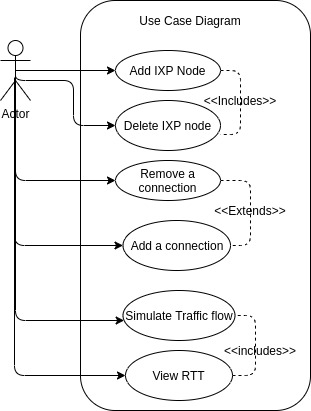
\includegraphics[width=8.5cm]{sections/pictures-diagrams/usecasedigarma.jpg}
   \caption{Use case diagram for the system.}
    \label{figure:galaxy}
\end{figure}

\subsubsection{Package diagram}
\begin{figure}[htp]
   \centering
     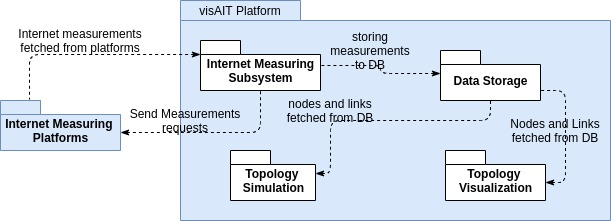
\includegraphics[width=10cm]{sections/pictures-diagrams/Package-Diagrma-v2.jpg}
   \caption{Package diagram showing various subsystems of the platform.}
    \label{figure:galaxy}
\end{figure}
The package diagram is used to show subsystems of a system on a high level. The package diagram we designed is illustrated in Figure 2 and it was used to visualize how various subsystems of the platform will depend and interact with each other. The diagram also showed how the system will look like in a more modular manner. 

The topology simulation subsystem depends on other three subsystems namely: Internet measuring subsystem,  topology visualization subsystem and Data Storage. Internet measuring platforms is an external package since the internet measuring platforms runs independently from our system. our system only interacts with the internet measuring platforms via API calls when measurements requests are sent by the internet measuring subsystem. The data storage subsystem stores data that has been collected by the internet measuring subsystem. The topology simulation and topology visualization subsystems interacts with the data storage to access the links and nodes' information that is stored in the data storage. 

\subsubsection {State Machine diagram}
State machine diagram illustrated in Figure 3 shows the various states the internet topology may be during simulation. The diagram shows how the topology transitions from one state to another when an event happens.

During pre-simulation phase, the topology is in idle state. When an node is removed from topology, the remove node method is invoked and the topology will transition to the state where the topology is shown without the removed node. When an IXP node is added to the topology, the add IXP node method is invoked and the topology transition to the state where the topology is shown with the added node. When a connection between two nodes is added to the topology, the add connection method is invoked and the topology transition to the state where the topology is shown with the added connection. When a connection between two nodes is removed from the topology, the remove connection method is invoked and the topology transition to the state where the topology is shown without the removed connection.

At any given state, the simulate traffic method can be invoked and the topology will transition to the state where the routing route and the link delay is shown. This was important as any action done on the internet topology could be evaluated of its effect on internet performance. 
\begin{figure*}
    \begin{center}
        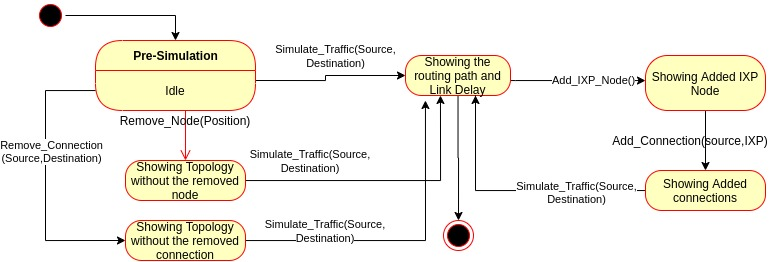
\includegraphics[width=1\linewidth]{sections/pictures-diagrams/sequence.jpg}
    \end{center}
    \caption{Diagram showing various states the topology may be during simulation}
    \label{figure:state}
\end{figure*}
\subsubsection{Link Delay and Routing Algorithm design}
Link delay is the metric used to determine performance of the scenario being tested during simulation is. Since every link is associated with link delay, the challenge was how to assign link delay to the new introduced links. According to Günther \textit{et al}\cite{RTTT}, the minimum Round Trip Time(RTT) internet traffic takes from a source to destination can be computed as: 
\begin{equation}
RTT(min) = 2*d/c
\end{equation}
\textit{where d is the distance 
between the source and the destination and c is the speed of light which is: }
\begin{equation}
c = 3*10^8
\end{equation}

We adopted this method to assign the link delays of the newly introduced connections during simulation. 

To determine the best route of internet traffic from source to destination, we implemented the Dijkstra's algorithm\cite{SaeediMEJ10} to determine the shortest distance between the source and the destination.  
	\section{SYSTEM DEVELOPMENT}\label{sec:system-development}
\subsection{System development methodology}\label{subsec:implementation-and-ui-design}
The development of this project took an agile and iterative approach of system development. This was to ensure that any changes proposed by the users or feedback given by the users could be incorporated in the development of the project.  Scrum was used as a project management method where the project was divided into 8 weekly sprints. After every sprint, the development team could meet to track the progress of  the development and choose the tasks that needed to be done in the following sprint.  The team project leader was also the scrum master who was responsible for ensuring that the team was in constant communication with users for effective system development and also in-charge of the whole scrum process. 

The project underwent various iterations where after every iteration feedback was given. 
\subsection{System Architecture}\label{subsec:system architecture}
The system was developed using the client-server architecture as shown in Figure 6 in the Appendix. This was to ensure that the platform could be accessed remotely. During run time, the simulator and visualizer components of the system could connect with the MongoDB online server where the database operations were running on. 

The system is made up of 5 main components namely: system web view, internet measuring platforms, internet measurements collector, databases and the database server. System web view is the user interface of the system which contains both the simulator and the visualizer. The web view provides the user with the functionality to view and simulate the Africa internet topology. The internet measurements collector collects traceroute measurements from the internet measuring platforms namely: CAIDA, RIPE and Speedchecker. The collection component contains a python script which runs after every three hours and collects internet measurements from three measuring platforms. 

The database server has four components namely: data mapper, query manager, request handler and the response handler. The data mapper maps and structure the data collected in order to be stored in the databases. The query manager handles the various queries sent to the databases. The request and the response handlers manages the data requests and responses sent to and from web view to the databases.

The system has two databases namely: traceroute database and nodes and links database. The traceroute database stores the traceroute measurements from the different measuring platforms while the nodes and links database stores data on links and the nodes. Since to plot the internet topology nodes and links are needed, the traces stored in the traceroute database were used to model links and nodes. The modelled links and nodes were stored separately from the traces to ensure that when the client wants to visualize or simulate internet topology, nodes and links could be loaded faster. To allow flexibility of our database and higher availability, both databases that were developed are noSQL.  

\subsection{Class Diagram}
Three classes were developed namely: node, link and weighted graph. The class diagram in Figure 4 shows the classes and the relationships between them. The node class is responsible for storing information about the ASN and IXP. The information stored includes the node number, type of the node and the geographical position of the node.  The link class is responsible for storing information about links between the nodes. The information stored includes the source node, target node and the link delay. The weighted graph class is responsible for storing all information about the nodes and links. The weighted class implements the Dijkstra's algorithm which is used to determine the shortest route between two nodes. 
\begin{figure}[htp]
   \centering
     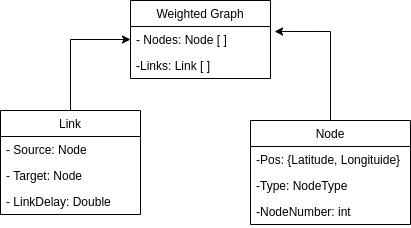
\includegraphics[width=8cm]{sections/pictures-diagrams/class-diagram.jpg}
   \caption{Class diagram for the system.}
    \label{figure:galaxy}
\end{figure}


\subsection{Framework and Technologies used}
The development of the system used various technologies in both front-end and the back-end. The python flask web framework was used to handle the front-end and back-end. The framework was used as it provided web tools and various python libraries which were necessary during the platform development which made the development easier as we could concentrate more on building the application rather than worrying how the dependencies will integrate. 

The web-view which forms the user interface was developed using HTML and CSS which are web markup and styling languages. JavaScript was used to script the functions that handled the events that occurred when various HTML components were clicked. To provide geographical mapping, the Google maps API was used for manipulating the Google Maps presented on the simulator. The D3 JavaScript library was also used to ensure good zooming and panning of the geographical maps. 

The back-end of the system was developed to run on the MongoDB online. MongoDB is a NoSQL online database which stores data in documents. This was necessary as we we dealt heavily with unstructured data that was collected from the internet measuring platforms. MongoDB also offers high availability of the data as it stores the data in three replicas ensuring that database queries can withstand fault tolerance. MongoDB also offers an option whereby you can connect the online database with a python application which made it easier for us to integrates the database with the rest of the application.  

The main python libraries that were used includes pymongo which was used to perform the database queries, geoIP2 database which was used to resolve the geo-location of a node given an IP address of the node, and the web-driver manager which is a library used to automate the management of web binaries. 

\subsection{System Testing}
System testing was done to evaluate whether the platform that was developed managed to achieve both functional and non-functional user requirements. The three types of testing that were carried are: usability testing, unit testing and functionality testing.
\subsubsection{Usability Testing}
10 users were selected to test the usability of the system. The users had background in networking and hence possible future users. During each test, users were asked to complete 5 uses cases using the simulator and answer if the simulator was useful and how easier it was to carry out the uses cases. 

"Add Node" and "Delete Node" use cases were the easiest as on average users took 1 minute to complete each tasks. The rest of the use cases took longer than 90 seconds to complete.

8 users agreed that the design of the simulator was okay but it needed improvement on three uses cases: "Add connection", "Remove connection" and "Simulate Traffic and View RTT". They pointed out the format of inputting the source and destination locations was not good enough. From this feedback, we enabled an information window when user clicks a node to allow them obtain the source and destination locations easily. 
\subsubsection{Unit and Integration Testing }
Unit testing was being carried out after every sprint to ensure that all units of source code were working well and properly. Since agile methodology was used to develop this project, testing was done regularly to ensure that any changes or issues that arose from source code could be addressed well in advance to avoid integration errors at the end of the project. During testing, the flask development environment was being changed from development to production to test how the system would behave during production.

During week 4 of the project, we experienced errors and bugs after testing due to data migration from local storage to the online MongoDB. This was due to failure of the flask environment to resolve the IP address of the remote database. This meant that the data storage unit of the system was not integrating well with our application. We decided to resolve the bug before proceeding to the next sprint and we managed to get a python library called dnspython which could integrate with pymongo to resolve the IP address of the remote MongoDB.  
\subsubsection{Functionality Testing}
Functionality testing was done to test if the developed system had fulfilled its functional requirements. Test cases for each use case were carried out as illustrated in the appendices. Test case for "Add IXP node" use case is illustrated in Figure 8. Test case for "Add Connection" use case is illustrated in Figure 9. Test case for "Delete node" use case is illustrated in Figure 10. Test case for "Delete Connection" use case is illustrated in Figure 11. Test case for "Simulate Traffic" and "View RTT" use cases illustrated in Figure 12. 

	\section{RESULTS AND DISCUSSION}\label{sec:results-and-discussion}
The results illustrated in this section focuses on three scenarios on which Africa's internet topology was simulated. During simulation, link delay which in this project we considered it as the minimum round trip time(RTT) was recorded for each source ASN - destination ASN pair for comparison and evaluation purposes to evaluate which scenario is the best African ISPs can peer at African IXPs. The three scenarios are: pre-simulation scenario where there is no IXP present in the topology, a scenario where one central IXP was added to the topology and a scenario where five regional IXPs were added to the topology. 
 \begin{figure*}
  
    \begin{center}
        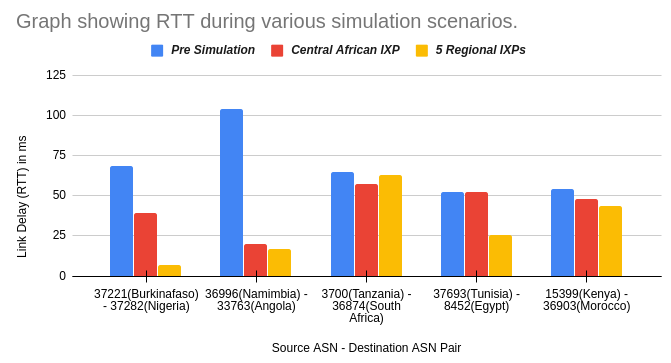
\includegraphics[width=1\linewidth]{sections/pictures-diagrams/graph22.png}
    \end{center}
    \caption{Graph showing RTT during various simulation scenarios.}
    \label{figure:state}
\end{figure*}
Five source ASN - destination ASN pairs were used as tabulated in Table 1. These pairs were chosen to represent the intra-continental Africa internet traffic traversing different regions across the continent. These pairs are namely: 37221(Burkinafaso) - 37282(Nigeria) representing internet traffic originating from ASN 37221 in Burkina Faso to ASN 37282 in Nigeria, 36996(Namimbia) - 33763(Angola) representing internet traffic originating from ASN 36996 in Namimbia to ASN 33763 in Angola, 3700(Tanzania) - 36874(South Africa) representing internet traffic originating from ASN 3700 in Tanzania to ASN 36874 in South Africa, 37693(Tunisia) - 8452(Egypt) representing internet traffic originating from ASN 37693 in Tunisia to ASN 8452 in Egypt and 15399(Kenya) - 36903(Morocco) representing internet traffic originating from ASN 15399 in Kenya to ASN 36903 in Morocco.

 \subsection{Scenarios}
 \subsubsection{Pre-Simulation}
 During this scenario, the topology had no IXP as shown in Figure 7 in the appendix. The scenario is called pre-simulation as it is the initial state of topology where initial measurements of the link delays are recorded for each source ASN - destination ASN. The readings recorded from this phase depicts the real link delays between the source ASN and the destination ASN. These reading are important as they form the base cases to discuss and compare how the link delay will be affected when other scenarios are tested. The results obtained from the pre-simulation phase are tabulated in Table 1. 
 
 \subsubsection{Simulating with a central African IXP}
In this scenario, a central African IXP was added to the topology. The IXP node was added in DRC which is in central Africa. We added the central IXP node in DRC since DRC is in Central Africa and central from all regions in Africa. After adding the IXP node, all source ASN and destination ASNs were connected to the newly introduced IXP. This can be seen well in Figure 13 in the appendix. After all connection had been added, traffic was simulated again to see the change of link delays. The results obtained are tabulated in Table 1.   
  
 \subsubsection{Simulating with 5 regional IXPs}
 In this scenario, 5 regional African IXP were added to the topology. Regional IXPs were added in Algeria for North Africa region, Ghana for West Africa region, Uganda for East Africa and Botswana for the Southern Africa region. These countries are regarded to be central amongst their respective regions. The IXP node that was added in DRC remained as it represented the Central Africa region. After adding the regional IXP nodes, all source ASN and destination ASNs were connected to their respective regional IXPs and all regional IXPs were finally connected to the central IXP node. This can be seen well in Figure 14 in the appendix. After all connections had been added, traffic was simulated again to see the change of link delays. The results obtained are tabulated in Table 1.

 \begin{table}[htp]
   \centering
     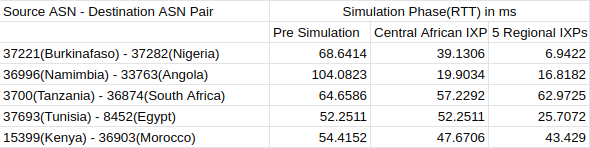
\includegraphics[width=8.5cm]{sections/pictures-diagrams/rttfigures.png}
   \caption{Table showing the RTT of different source ASN - destination ASN Pair when simulated in three scenarios .}
    \label{figure:galaxy}
\end{table}

\subsection{Discussion on the results}
From the graph shown in Figure 5, with the introduction of central African IXP, the link delay of each source ASN - destination ASN decreased by more than 50\% except for the 37639 ASN in Tunisia and 8452 ASN in Egypt. The most significant decrease is the 36696 ASN - 33753 pair due to their close proximity with DRC. The link delays for 37693 ASN - 8452 ASN pair did not decrease due to their presence in North Africa which is quite far from DRC. This scenario shows that, if African ISPs could peer at central Africa IXP located in Central Africa, only internet performance in the South, East, Central and some parts of West Africa Africa will improve. The internet performance in North Africa will still remain the same. Most of the West Africa ISPs peers at IXPs located in France and if they peer at central African IXP, inter-regional internet performance may improve as shown by the ASN 37221 (Burkinafaso) - ASN 37282 (Nigeria).

In the scenario where five regional IXPs were introduced in the topology, the regional internet performance improved highly as the link delay decreased by more than 75\% but also the inter-regional internet performance improved as the link delay dropped by 20\%. The inter-regional traffic is represented by traffic originating from 15399 ASN in Kenya to 36903 ASN in Morocco and 3700 ASN in Tanzania to 36874 ASN in South Africa.

This shows that African ISPs should peer at regional IXPs to ensure that regional internet performance is good and the regional IXPs should be connected to a central IXP to ensure that inter-regional internet performance also improves.  

	\section{ETHICAL, PROFESSIONAL, AND LEGAL ISSUES}\label{sec:ethical,-professional,-and-legal-issues}
This project has been accorded the Creative Commons License to ensure that the work can be used by the open source community to create tools to conduct internet research. This was inspired by the usage of many open source tools such as python libraries, python flask web framework to develop the system. 

The project do not use any sensitive data of the user as it purely runs online where the user do not need to create an account or prior installation when using the system. 
	\section{CONCLUSION AND FUTURE WORK}\label{sec:conclusion}
This work has defined the development of an online internet topology simulator. The simulator was used to simulate Africa's internet topology to evaluate two peering scenarios which African ISPs can peer. African ISPs peering at regional IXPs turns out to be the best scenario where the African ISPs could peer as the regional internet latency drops by 75\% and the inter-regional internet latency drops by 20\%. 

This work only considered the geographical position of an ISP to evaluate the peering scenario. However, there are various factors that affects ISP peering such as language spoken in a country, economic status of an ISP. Future work of this work should focus on integrating these factors in modelling the simulation algorithm to ensure that simulation results obtained are inclusive of all factors that affect ISP peering. 

\subsection{ACKNOWLEDGEMENTS}
I would like to acknowledge the other project team members: Blessed Chitamba and Gerald Ngumbulu for their immense support and contributions to development of this project and to Dr. Josiah Chavula for guiding us throughout the project. I would also acknowledge Professor James Gain for his input also during the first demo of the project and giving insights on how we could improve our project proposal.   




	\bibliographystyle{acm}
	\bibliography{references}
	\appendix
\appendixpage
\begin{figure*}
    \begin{center}
        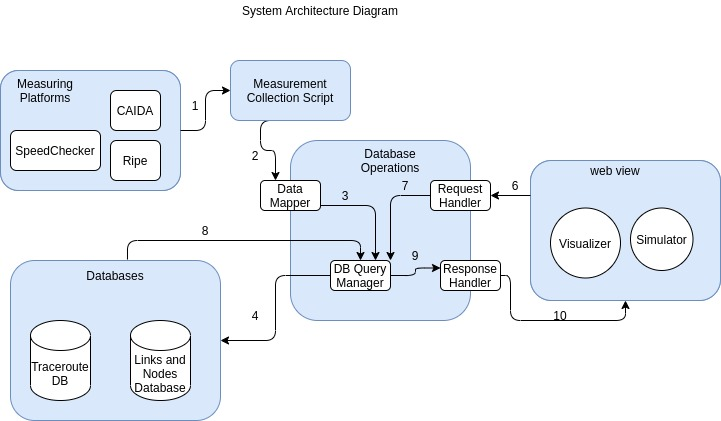
\includegraphics[width=1\linewidth]{sections/pictures-diagrams/system architecture (1).jpg}
    \end{center}
    \caption{ System architecture diagram showing various components of the system.}
    \label{figure:state}
\end{figure*}

\begin{figure*}
    \begin{center}
        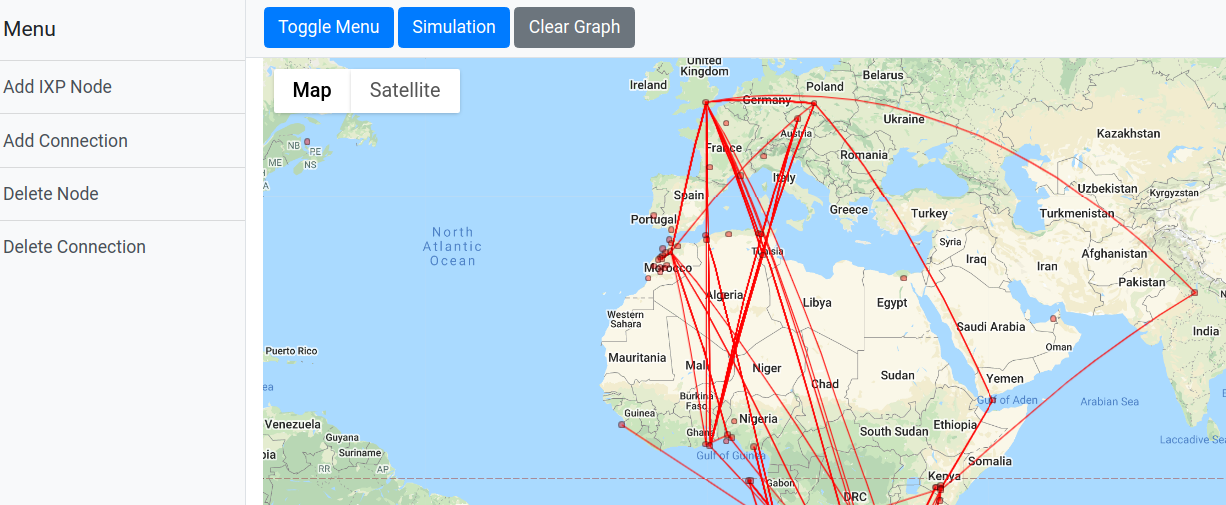
\includegraphics[width=1\linewidth]{sections/pictures-diagrams/original picture.png}
    \end{center}
    \caption{Picture showing initial topology before simulation}
    \label{figure:state}
\end{figure*}

\begin{figure*}
    \begin{center}
        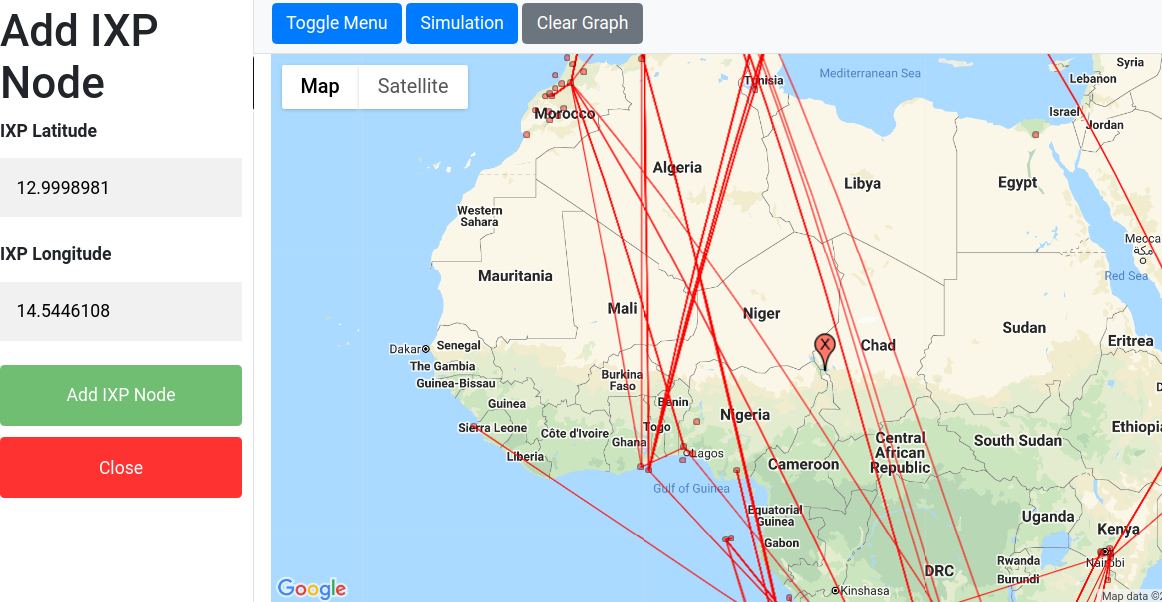
\includegraphics[width=1\linewidth]{sections/pictures-diagrams/Addnode-picture.png}
    \end{center}
    \caption{Picture showing the adding node functionality testing.}
    \label{figure:state}
\end{figure*}

\begin{figure*}
    \begin{center}
        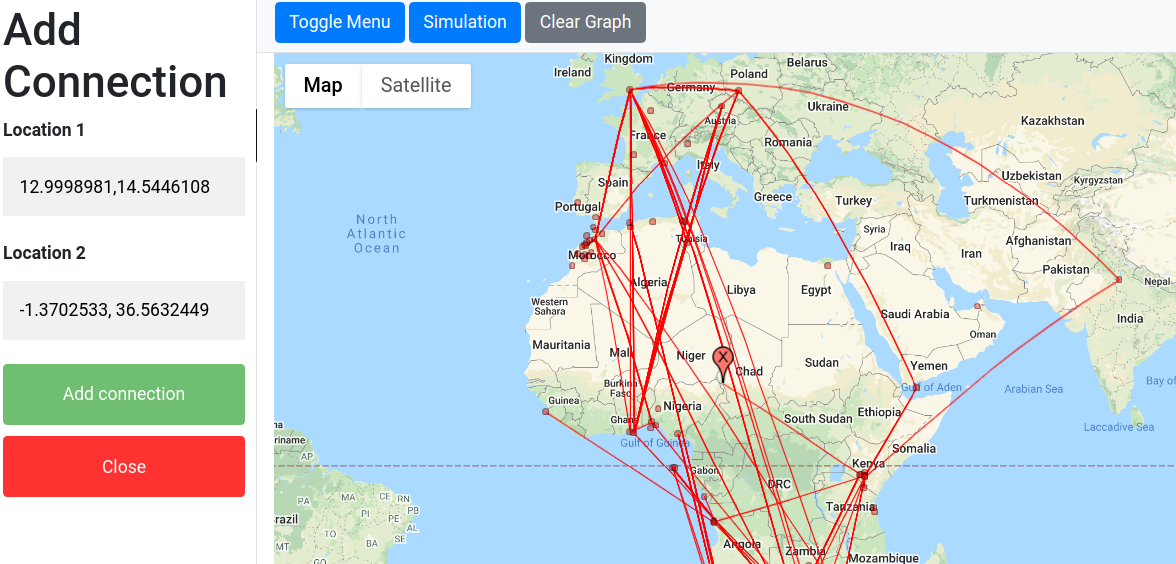
\includegraphics[width=1\linewidth]{sections/pictures-diagrams/addconnection.png}
    \end{center}
    \caption{Picture showing the adding connection functionality testing.}
    \label{figure:state}
\end{figure*}
\begin{figure*}
    \begin{center}
        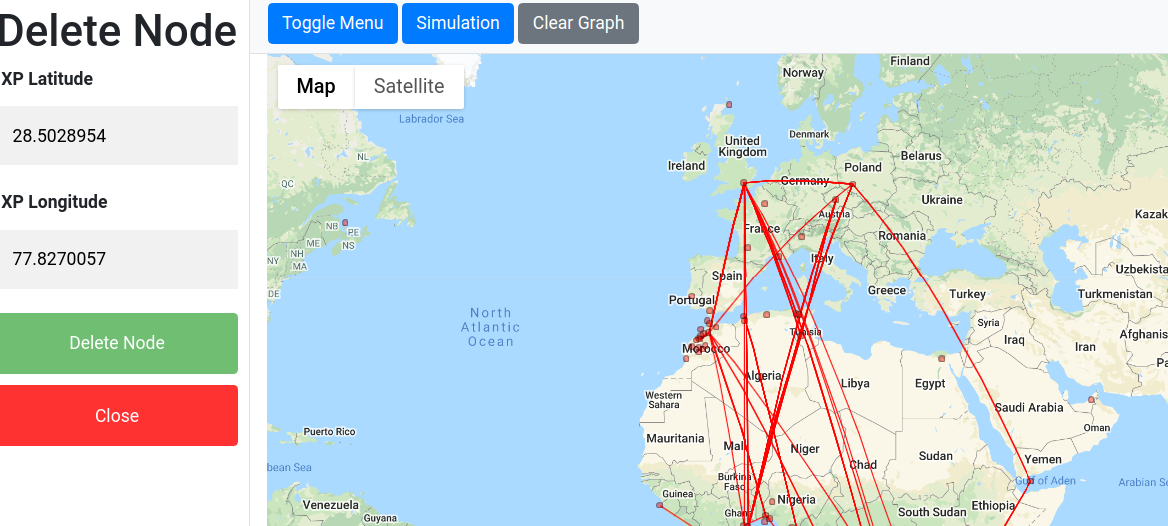
\includegraphics[width=1\linewidth]{sections/pictures-diagrams/deletenodepicture.png}
    \end{center}
    \caption{Picture showing the delete node functionality testing.}
    \label{figure:state}
\end{figure*}
\begin{figure*}
    \begin{center}
        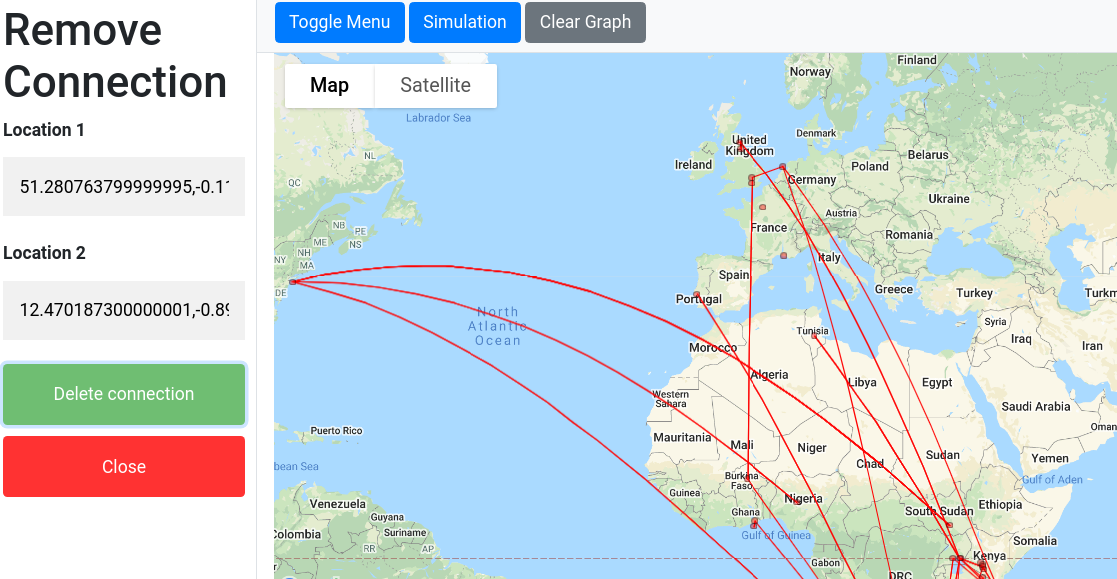
\includegraphics[width=1\linewidth]{sections/pictures-diagrams/removeconnection.png}
    \end{center}
    \caption{Picture showing the delete connection functionality testing.}
    \label{figure:state}
\end{figure*}
\begin{figure*}
    \begin{center}
        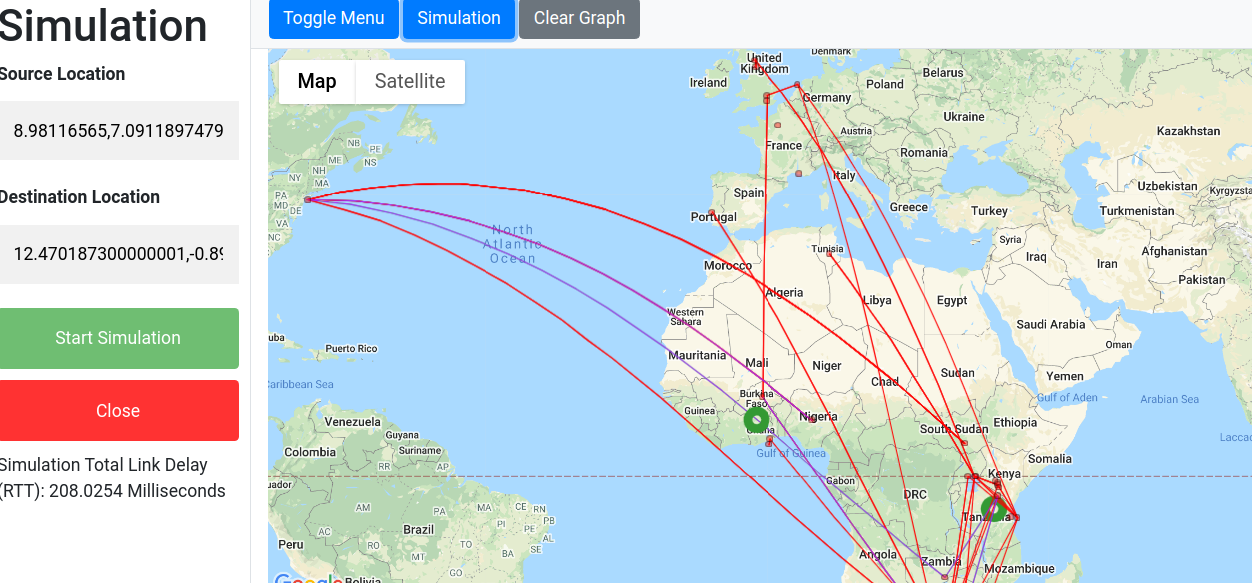
\includegraphics[width=1\linewidth]{sections/pictures-diagrams/simulateandrttpicture.png}
    \end{center}
    \caption{Picture showing the Simulating traffic and viewing RTT functionality testing.}
    \label{figure:state}
\end{figure*}
\begin{figure*}
    \begin{center}
        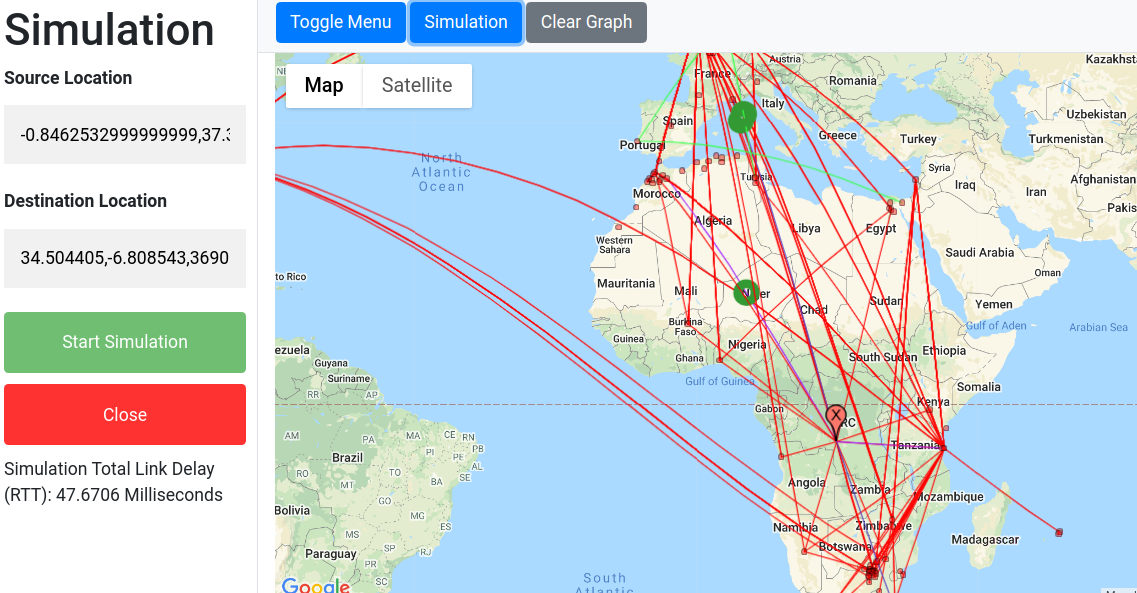
\includegraphics[width=1\linewidth]{sections/pictures-diagrams/OneIXPAdded.png}
    \end{center}
    \caption{Picture showing the simulation done with one IXP added in DRC.}
    \label{figure:state}
\end{figure*}
\begin{figure*}
    \begin{center}
        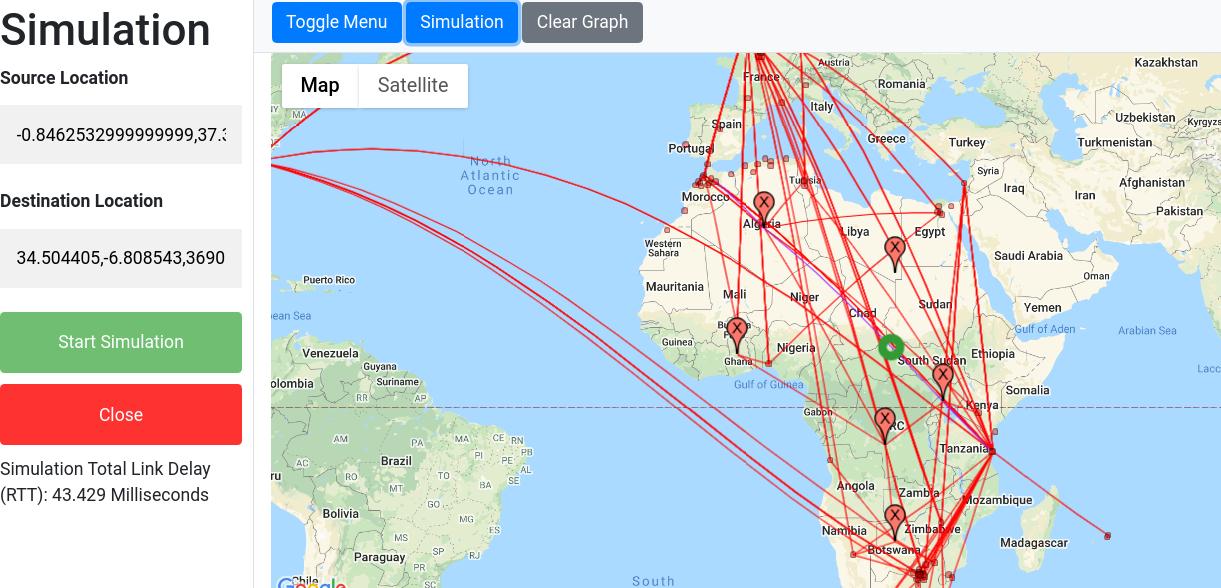
\includegraphics[width=1\linewidth]{sections/pictures-diagrams/5regionalIXPnodesadded.png}
    \end{center}
    \caption{Picture showing the simulation done with 5 regional IXPs added in Uganda, Botswana, Ghana and Algeria}
    \label{figure:state}
\end{figure*}
\begin{figure*}
		\centering
		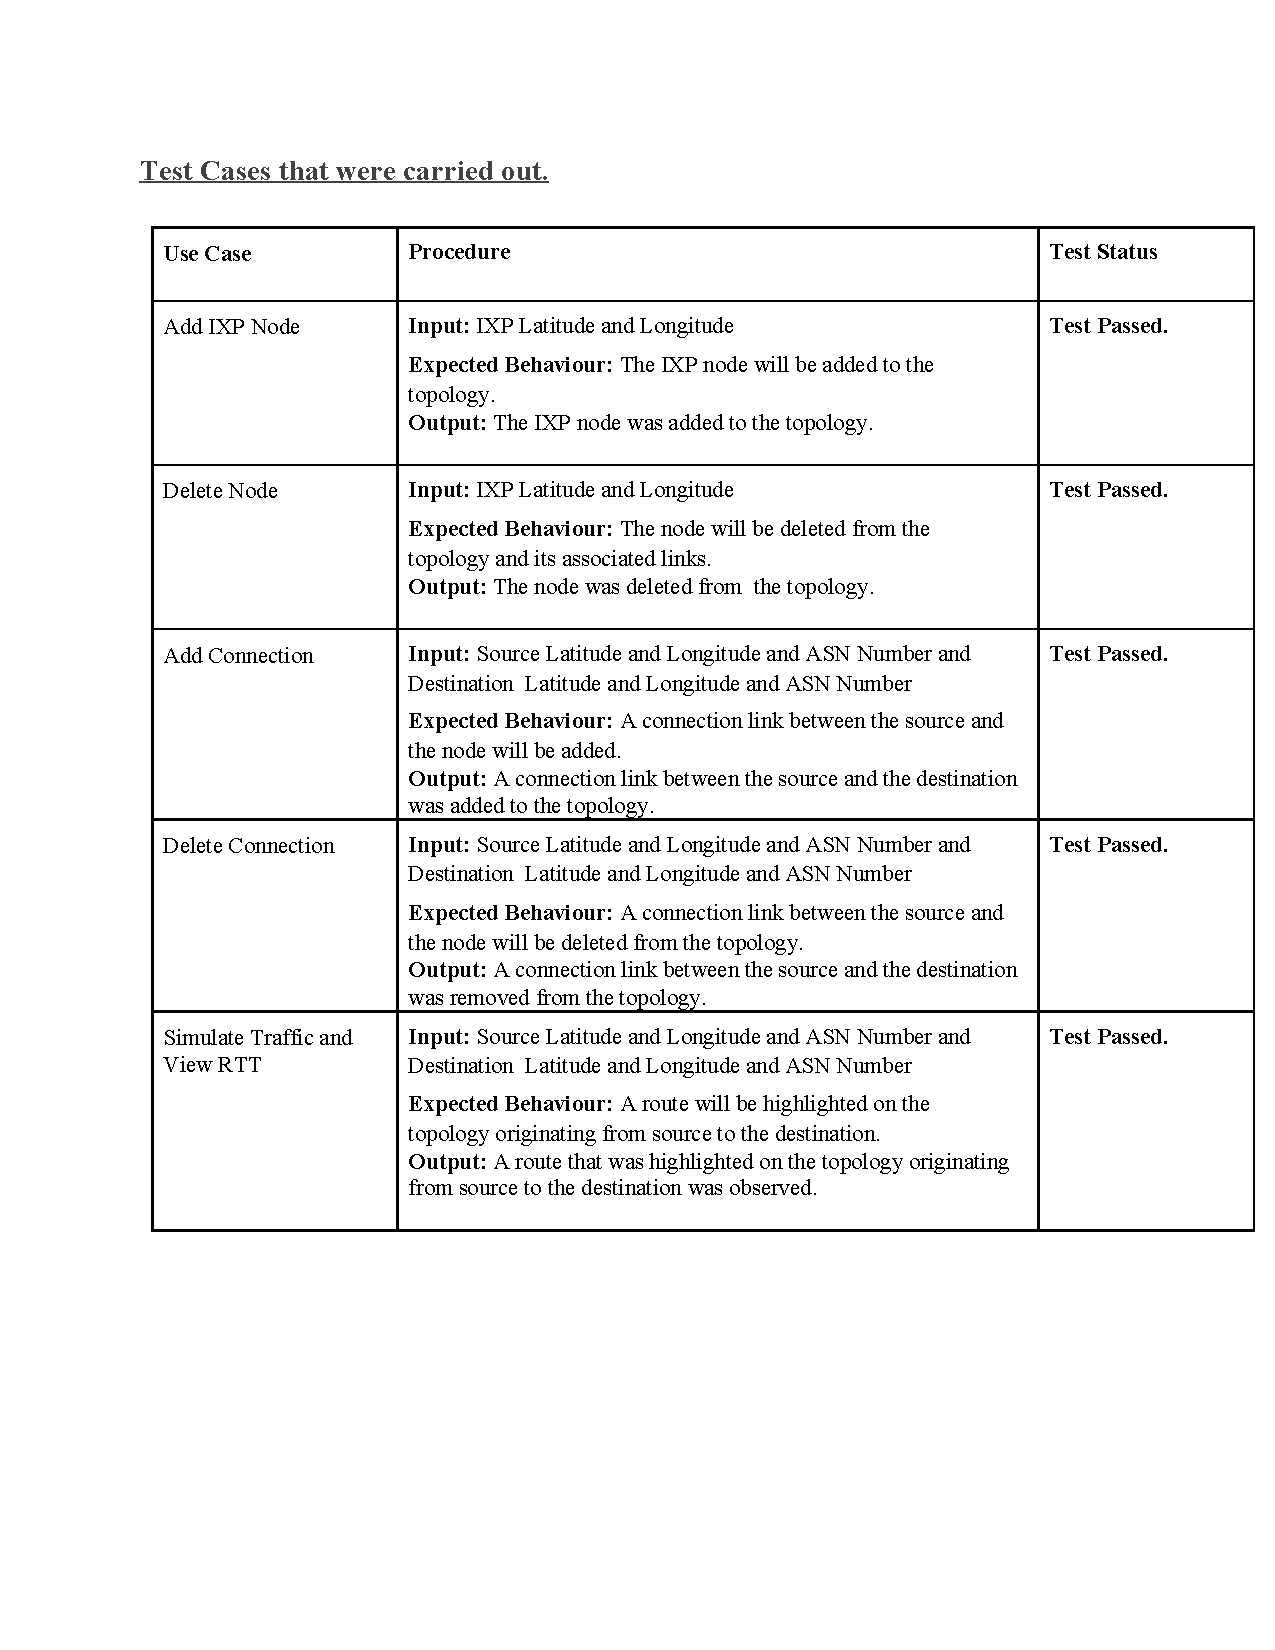
\includegraphics[width=1\linewidth]{Testing procedures.docx.pdf}
		\caption{Table showing the test cases that were carried out.}
		 \label{figure:state}
	\end{figure*}
\end{document}